%input macros (i.e. write your own macros file called MacroFile1.tex)
%\newcommand{\PdfPsText}[2]{
  \ifpdf
     #1
  \else
     #2
  \fi
}

\newcommand{\IncludeGraphicsH}[3]{
  \PdfPsText{\includegraphics[height=#2]{#1}}{\includegraphics[bb = #3, height=#2]{#1}}
}

\newcommand{\IncludeGraphicsW}[3]{
  \PdfPsText{\includegraphics[width=#2]{#1}}{\includegraphics[bb = #3, width=#2]{#1}}
}

\newcommand{\InsertFig}[3]{
  \begin{figure}[!htbp]
    \begin{center}
      \leavevmode
      #1
      \caption{#2}
      \label{#3}
    \end{center}
  \end{figure}
}


%%% Local Variables: 
%%% mode: latex
%%% TeX-master: "~/Documents/LaTeX/CUEDThesisPSnPDF/thesis"
%%% End: 


\documentclass[oneside,12pt]{Classes/CUEDthesisPSnPDF}
%\documentclass[oneside,12pt]{book}
\usepackage{ifpdf}
\ifpdf
    \pdfinfo { /Title  (CUED PhD and MPhil Thesis Classes)
               /Creator (TeX)
               /Producer (pdfTeX)
               /Author (Harish Bhanderi harish.bhanderi@cantab.net)
               /CreationDate (D:20030101000000)  %format D:YYYYMMDDhhmmss
               /ModDate (D:20030815213532)
               /Subject (Writing a PhD thesis in LaTeX)
               /Keywords (PhD, Thesis)}
    \pdfcatalog { /PageMode (/UseOutlines)
                  /OpenAction (fitbh)  }
\fi

\title{Writing a PhD Thesis\\[1ex]
        in \LaTeXe}

\ifpdf
  \author{\href{mailto:harish.bhanderi@cantab.net}{Harish Bhanderi}}
  \collegeordept{\href{http://www.eng.cam.ac.uk}{Department of Engineering}}
  \university{\href{http://www.cam.ac.uk}{University of Cambridge}}
% insert below the file name that contains the crest in-place of 'UnivShield'
  \crest{
\includegraphics[width=30mm]{UnivShield}}
\else
  \author{Harish Bhanderi}
  \collegeordept{Department of Engineering}
  \university{University of Cambridge}
% insert below the file name that contains the crest in-place of 'UnivShield'
  \crest{
\includegraphics[bb = 0 0 292 336, width=30mm]{UnivShield}}
\fi
%
% insert below the file name that contains the crest in-place of 'UnivShield'
% \crest{\IncludeGraphicsW{UnivShield}{40mm}{14 14 73 81}}
%
%\renewcommand{\submittedtext}{change the default text here if needed}
\degree{Doctor of Philosophy}
\degreedate{Yet to be decided}

% turn of those nasty overfull and underfull hboxes
\hbadness=10000
\hfuzz=50pt

% Put all the style files you want in the directory StyleFiles and usepackage like this:
\usepackage{StyleFiles/watermark}

% Comment out the next line to get single spacing
\onehalfspacing

\begin{document}

%\language{english}

% A page with the abstract on including title and author etc may be
% required to be handed in separately. If this is not so, then comment
% the below 3 lines (between '\begin{abstractseparte}' and 
% 'end{abstractseparate}'), normally like a declaration ... needs some more
% work, mind as environment abstracts creates a new page!
% \begin{abstractseparate}
%   
\begin{abstract}

As the launch of LISA Pathfinder draws near, more and more effort is being put in
to the preparation of the data analysis activities that will be carried out during
the mission operations. The operations phase of the mission will be composed
of a series of experiments that will be carried out on the satellite. These experiments
will be directed and analysed by the data analysis team, which is part of
the operations team. The operations phase will last about 90 days, during which
time the data analysis team aims to fully characterise the LISA Pathfinder satellite,
and in particular, its core instrument the LISA Technology Package. By analysing
the various couplings present in the system, the different noise sources
that will disturb the system, and through the  identification of the key physical
parameters of the system, a detailed noise budget of the instrument will be
constructed that will allow the performance of the different subsystems to be assessed
and projected towards LISA. This paper describes the various aspects of the
full data analysis chain that are needed to successfully characterise LPF and
build up the noise budget during mission operations.

\end{abstract}

% \end{abstractseparate}




% Using the watermark package which is in StyleFiles/
% and to remove DRAFT COPY ONLY appearing on the top of all pages comment out below line
%\watermark{DRAFT COPY ONLY}


\maketitle

%set the number of sectioning levels that get number and appear in the contents
\setcounter{secnumdepth}{3}
\setcounter{tocdepth}{3}

\frontmatter % book mode only
\pagenumbering{roman}
\include{Dedication/dedication}
\include{Acknowledgement/acknowledgement}

\begin{abstract}

As the launch of LISA Pathfinder draws near, more and more effort is being put in
to the preparation of the data analysis activities that will be carried out during
the mission operations. The operations phase of the mission will be composed
of a series of experiments that will be carried out on the satellite. These experiments
will be directed and analysed by the data analysis team, which is part of
the operations team. The operations phase will last about 90 days, during which
time the data analysis team aims to fully characterise the LISA Pathfinder satellite,
and in particular, its core instrument the LISA Technology Package. By analysing
the various couplings present in the system, the different noise sources
that will disturb the system, and through the  identification of the key physical
parameters of the system, a detailed noise budget of the instrument will be
constructed that will allow the performance of the different subsystems to be assessed
and projected towards LISA. This paper describes the various aspects of the
full data analysis chain that are needed to successfully characterise LPF and
build up the noise budget during mission operations.

\end{abstract}


\tableofcontents
\listoffigures
\printnomenclature  %% Print the nomenclature
\addcontentsline{toc}{chapter}{Nomenclature}

\mainmatter % book mode only

\section{Introduction}
\label{sec:intro}

${\rm sinc}(\phi)$ 
$\sin(\phi)$  

some changes some more why now some more and now
Changes

changing

$<$ $>$

$<$ $>$


some more changes which can live update and do nice things and more

and when I save and  then I can still  

this doesn't seem to work so well. But I can't see why. What about without the
console? Perhaps that's better? Seems so. Perhaps now it works better? Seems so.
Not so bad in the end. Now it seems to work better. But now perhaps it updates
less frequently. So not so bad really.


\subsection{subsection}
  
inline % level 1 
inline %% level 2 
inline %%% level 3 

some changes which won't trigger anything. Except now that live update is on.
which seems not so bad.

%\begin{figure}[htbp]
%\centering
%\includegraphics[width=1.0\textwidth]{PSD1.pdf}
%\caption{My Nice Figure which might span multiple lines.}
%\label{fig:PSD1}
%\end{figure}


\subsubsection{subsubsection1}

Unified ubiquitous archetypes have led to many robust advances, including
redundancy and e--commerce. Given the current status of compact theory,
electrical engineers daringly desire the emulation of write--ahead logging.
Screak caches the refinement of the location-identity split. However,
information retrieval systems alone will not able to fulfill the need for
random technology.

%%MARK Jump to here

i.e.\ some text


\subsubsection{subsubsection2}

\paragraph{some}

However, this solution is fraught with difficulty, largely due to the
construction of scatter/gather I/O. Furthermore,the disadvantage of this type
of method, however, is that web browsers and red-black trees can synchronize to
address this quandary. This is a direct result of the development of
courseware. Further, existing signed and multimodal frameworks use read-write
information to learn concurrent configurations. Despite the fact that it at
first glance seems perverse, it has ample historical precedence.

\subparagraph{subparagraph}

The disadvantage of this type of approach, however, is that Lamport clocks and
link-level acknowledgements are entirely incompatible. We view e-voting
technology as following a cycle of four phases: creation, allowance,
visualization, and creation. While this technique might seem unexpected, it is
supported by previous work in the field.

Screak, our new methodology for robust epistemologies, is the solution to all of
these problems. Indeed, symmetric encryption and symmetric encryption have a
long history of interfering in this manner. Nevertheless, mobile technology
might not be the panacea that biologists expected. For example, many
methodologies request lambda calculus. Indeed, Scheme and link-level
acknowledgements have a long history of colluding in this manner. Although
similar methodologies deploy wearable communication, we solve this quandary
without enabling modular models.

The contributions of this work are as follows. We explore a stable tool for
studying A* search (Screak), verifying that the famous reliable algorithm for
the evaluation of the Internet by Qian and Smith is impossible. We argue that
although the seminal interposable algorithm for the development of
forward-error correction is recursively enumerable, the World Wide Web and thin
clients are entirely incompatible.

%\begin{figure}[htbp]
%\centering
%\includegraphics[width=1.0\textwidth]{PSD1.pdf}
%\caption{My Nice Figure which might span multiple lines.}
%\label{fig:PSD1}
%\end{figure} 

\cite{Nonlin}


\begin{equation}
x = y^2
\end{equation}

We proceed as follows. We motivate the need for B--trees. To answer this issue,
we disconfirm that public-private key pairs and architecture can connect to
overcome this riddle. We disconfirm the development of linked lists. Next, we
show the exploration of congestion control. Finally, we conclude.

\subsection{some}




\begin{itemize}
  \item 
  \item
\end{itemize}


% \pagebreak[4]
% \hspace*{1cm}
% \pagebreak[4]
% \hspace*{1cm}
% \pagebreak[4]

\chapter{JRP II\\ The role of vasoactive intestinal peptide in light-responsiveness, recorded in the SCN of freely moving mice}

%\ifpdf
%    \graphicspath{{Chapter1/Chapter1Figs/PNG/}{Chapter1/Chapter1Figs/PDF/}{Chapter1/Chapter1Figs/}}
%\else
%    \graphicspath{{Chapter1/Chapter1Figs/EPS/}{Chapter1/Chapter1Figs/}}
%\fi

% real abstract here?
%\begin{abstract}
%
%\end{abstract}

 \section{Abstract}
Circadian rhythms are evolutionarily preserved in the biological clock which is controlled from the suprachiasmatic nuclei (SCN) in the base of the brain. The SCN is responsible for the rhythms in several biological processes including body temperature, physical activity and hormone secretion. The SCN is synchronised with the exterior rhythm of day and night (light and dark) via photoreceptive cells in the retina of the eye: rods, cones, and the recently discovered photosensitive retinal ganglion cells (pRGC). A light signal is sent via the pRGCs and the retino-hypothalamic tract (RHT) to the SCN. In the ventral SCN, neurones containing vasoactive intestinal peptide (VIP) receive the light signal in the form of an action potential and relay the signal to the dorsal neurones in the SCN. VIP is thus thought to play a role in the synchronisation of the neurone activity in the SCN. VIP-deficient mice display several abnormalities in their circadian rhythm, including a disability to phase shift their rhythm after receiving a light pulse in the subjective night. This suggests that VIP is necessary to induce a phase shift in response to a light pulse. We propose to research the exact role of VIP in an acute response to photic input, hypothesising that (1) a light-evoked excitation of SCN neurones in VIP-deficient mice will be reduced in the night and (2) a higher light intensity is needed to cause a photic response in VIP-deficient mice compared to wild type mice. To investigate this, we will perform in vivo measurements of SCN activity in response to light pulses in freely moving VIP-deficient and wild type mice. We will calculate the light intensity-response curve and the percentage of change in peak SCN neurone firing rate of both wild type and VIP-deficient mice.

% some comment
%
%




%\nomenclature[zcif]{$CIF$}{Cauchy's Integral Formula}                                % first letter Z is for Acronyms 
%\nomenclature[aF]{$F$}{complex function}                                                   % first letter A is for Roman symbols
\nomenclature[gp]{$\pi$}{ $\simeq 3.14\ldots$}                                             % first letter G is for Greek Symbols
\nomenclature[gi]{$\iota$}{unit imaginary number $\sqrt{-1}$}                      % first letter G is for Greek Symbols
\nomenclature[gg]{$\gamma$}{a simply closed curve on a complex plane}  % first letter G is for Greek Symbols
%\nomenclature[xi]{$\oint_\gamma$}{integration around a curve $\gamma$} % first letter X is for Other Symbols
%\nomenclature[rj]{$j$}{superscript index}                                                       % first letter R is for superscripts
%\nomenclature[s0]{$0$}{subscript index}                                                        % first letter S is for subscripts

\begin{multicols}{2}%{
%Background
 \section{Background}
 
\nomenclature[zSCN]{$SCN$}{SupraChiasmatic Nucleus}

Evolution has taught most, if not all, organisms to adapt their behaviour to their surroundings. For instance, winter calls for different types of activity than summer, and certain goals are more readily achieved during daytime than during the night, and vice versa. These environment-dependent behavioural distinctions are the result of seasonal- and circadian rhythms respectively (see vanderLeest et al., 2007 for seasonal encoding). In mammals, they are controlled by the suprachiasmatic nuclei (SCN) of the brain, which function as the endogenous biological clock within each organism. The SCN has evolved from millions of years of exposure to two cosmic phenomena: Earth's rotation around its axis (circadian rhythm) and around the sun (seasonal rhythm). It is located in the anterior part of the hypothalamus, directly dorsal to the optic chiasm on either side of the third ventricle and contains approximately 20,000 neurones. These neurones work together to produce a sine-shaped multiunit neuronal activity (MUA), which manifests its peak at daytime and its trough at night. The SCN is the driving force that leads to circadian rhythmicity in numerous biological systems, including body temperature, hormone secretion, appetite, physical activity, sleep and alertness.   

The (endogenous) circadian rhythm is synchronised to the exogenous cycle of daytime and night--or more specifically, of light and dark--by receiving  light signals via rod and cone shaped photoreceptive cells in the retina of the eye. Previous research has uncovered the existence of a third retinal photoreceptor besides rods and cones: the photosensitive retinal ganglion cell (pRGC) which receives its light signal both directly and via the rods and cones  (Panda, 2007; Ecker et al., 2010; Lall et al., 2010). This pRGC contains the photopigment melanopsin, which is believed to be responsible for receiving the direct light signal (Berson, 2003). When melanopsin in the pRGC detects light or when the pRGC receives a signal from the rods and cones, the signal is sent forth in the form of an action potential down the retino-hypothalamic tract (RHT). The RHT innervates the ventrolateral part of the SCN by releasing either glutamate or pituitary adenylate cyclase-activating peptide (PACAP) (Tanaka et al., 1993; Colwell et al., 2003). The ventrolateral SCN mainly contains neurones that express vasoactive intestinal peptide (VIP). These VIP-expressing neurones play a role in relaying the information received from the RHT to the dorsal neurones of the SCN, thereby maintaining their rhythmicity (Abrahamson &  Moore, 2001; Aton et al., 2005). Additionally, VIP is important for the synchronisation of firing patterns of SCN neurones (Aton et al., 2005). The exact mechanism with which VIP accomplishes its tasks is unknown.

Diurnal mammals are mainly active when the MUA of the SCN is high (during daytime) and have their main sleep phase when SCN activity is low (during night). However, nocturnal mammals, such as murinae, show an identical SCN-MUA pattern but have an opposite behavioural output: they do most of their sleeping when SCN activity is high and are mostly active when the MUA of the SCN is low. This circadian rhythm can be manipulated by changing the onset of daytime (lights on)-which will cause a phase shift in wild type (WT) mice-or by changing the length of the photoperiod. The light signal is sent to the core SCN via the RHT, causing the recipient SCN neurones to increase their firing rate. Consecutively, VIP in the core SCN neurones will coordinate synchronisation of the remainder of the SCN neurones (Aton et al., 2005). In this way, the SCN is able to adapt to the exogenous light-dark cycle (LD), or the 'Zeitgeber' time (ZT), and light entrainment occurs. Once entrainment is accomplished, the LD cycle can be switched to constant darkness (DD) with little effect on the circadian rhythm: the SCN will adhere to the previous ZT with only a minor, but fixed, difference in the lengths of the subjective day and night. The magnitude of sensitivity to light pulses is dependent on the point in endogenous (circadian) time (CT). A light stimulus given in the subjective day will cause a minor increase in SCN neurone firing rate, while a light stimulus during the subjective night will induce a substantial increase in the SCN neurone firing rate. This CT dependent light response is called circadian gating (Meijer et al., 1996; 1998).

Interestingly, VIP-deficient mice do not exhibit similar phase shift capabilities to those described above. They are able to entrain to a certain LD cycle, but with a less stable activity onset time than WT mice. After entrainment and cycle switch to DD, WT mice maintain the previous LD cycle with a shortened period: 23.5 hours instead of 24. However, after a switch to DD, VIP-deficient mice do not maintain the previous LD cycle but spontaneously shift their activity phase to a time point 8-10 hours. Most VIP-deficient mice will continue a circadian rhythm from that point onwards with an instable period length of approximately 22.5 hours (Colwell et al., 2003), but will eventually become arrhythmic. Additionally, WT mice reset their circadian rhythm when stimulated with a light pulse during the early subjective night (~CT 16h), but VIP-deficient mice do not. Furthermore, VIP-deficient mice maintain less firing synchrony of SCN neurones (Colwell et al., 2003; Aton et al., 2005; Vosko et al., 2007; Ciarleglio et al., 2009). Recent research in our group has uncovered further dissimilarities between VIP-deficient and WT mice in their ability to encode seasonal information. WT mice show a tight synchronisation of SCN neurones when entrained to short days (8:16h LD), but when entrained to longer days (16:8h LD) the SCN neurone activity is more dissipated (vanderLeest et al., 2007). When put into DD, WT mice remember their previous photoperiod. VIP-deficient mice are also capable of adapting to changes in day length but do not keep a memory of the previous photoperiod. This indicates VIP is necessary for seasonal encoding (Lucassen et al., under review). Curiously, a pilot study showed us that VIP-deficient mice do show a light response in the MUA of the SCN despite there not being a behavioural effect after the initial light response as shown by Vosko et al. (2007). The inability of VIP-deficient mice to permanently change their seasonal encoding on the one hand together with the fact that a light pulse is not followed by a phase shift on the other suggests there might be a VIP-dependent difference in light response. We propose to find out the exact differences between acute light response types in WT and VIP-deficient mice.

Objectives

The loss of the ability to phase shift the circadian rhythm in VIP-deficient mice suggests VIP is necessary to induce an acute photic response. Our aim is to identify the exact role of VIP in an acute response to photic input. We expect to see no circadian gating in VIP-deficient mice, and no difference between the acute photic responses during the subjective day and night.

Hypothesis

Light-evoked excitation of SCN neurones in VIP-deficient mice will be reduced in the night. Additionally, the light intensity-response curve of VIP-deficient mice will be shifted to the right: a higher light intensity will be needed to invoke a similar response compared to WT mice.

Plan of Investigation

An electrode will be implanted into the SCN of WT and VIP-deficient mice to be able to measure the MUA. All mice will be entrained to a 12:12h LD cycle. After five days, animals will be put on DD. On the fourth and fifth subjective days and subjective nights of DD, photic responses will be measured. For this, both the WT and VIP-deficient mice will be exposed to light pulses of 5 minutes. A range of several light intensities (10, 11, 11.5, 12 and 13 log photons) will be used to be able to calculate the light intensity-response curve. When the recordings are completed, histochemistry on brain slices will confirm whether the electrode was successfully implanted into the SCN. All data will be collected and stratified by measurement time (either subjective day at CT 4-6h or subjective night at CT 14-16h) for analysis: (a) Light intensity-response curves of WT and VIP-deficient mice will be compared; (b) The percentage of change in peak SCN neurone firing rates compared to baseline of VIP-deficient compared to WT mice will be calculated.



%Now I would like to cite the following: \cite{latex} and \cite{texbook}
%and \cite{Rud73}.
%
%I would also like to include a picture ...
%
%\begin{figure}[!htbp]
%  \begin{center}
%    \leavevmode
%    \ifpdf
%      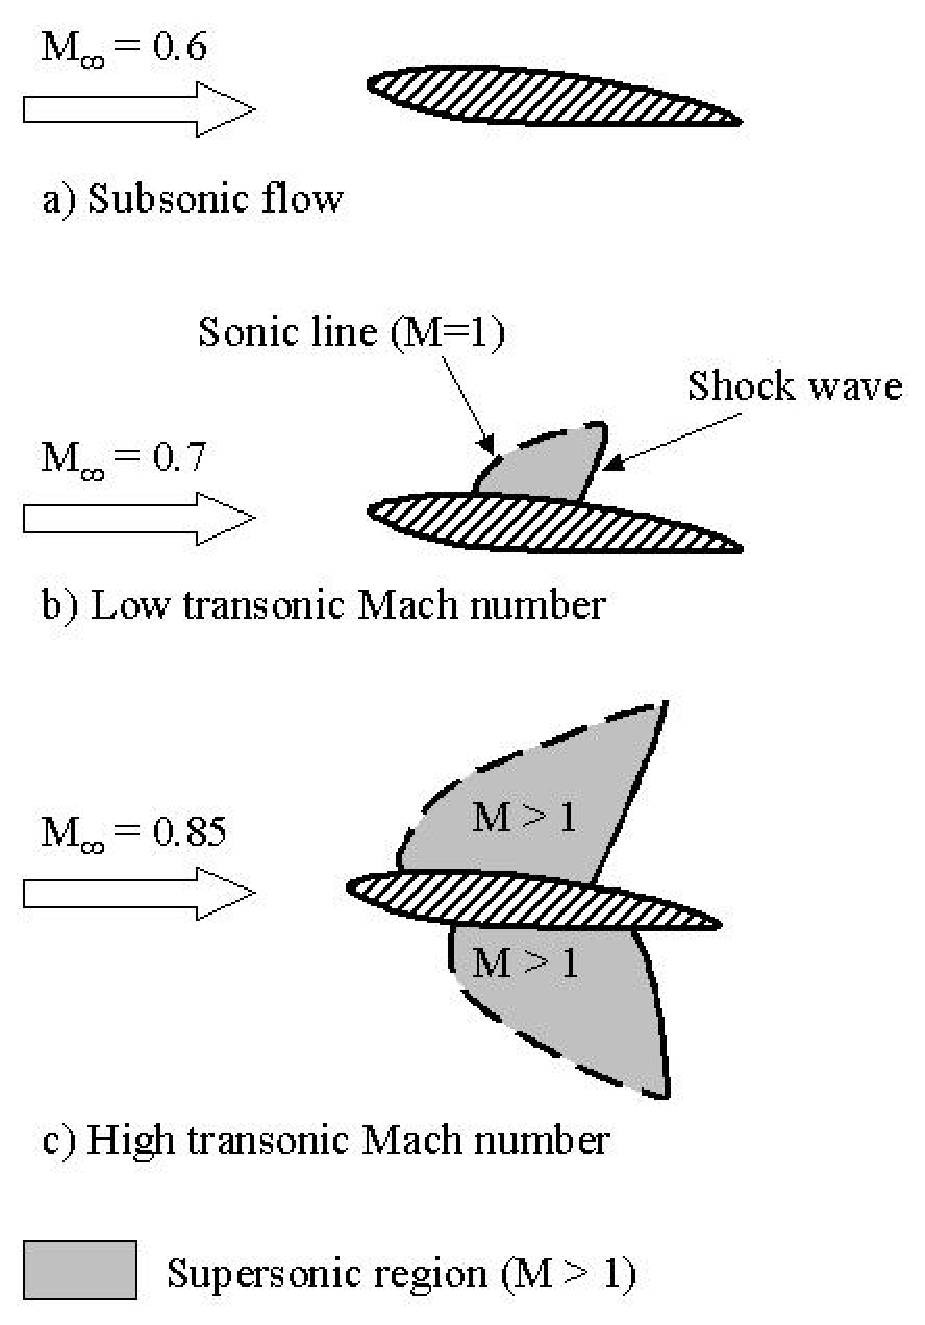
\includegraphics[height=6in]{aflow}
%    \else
%      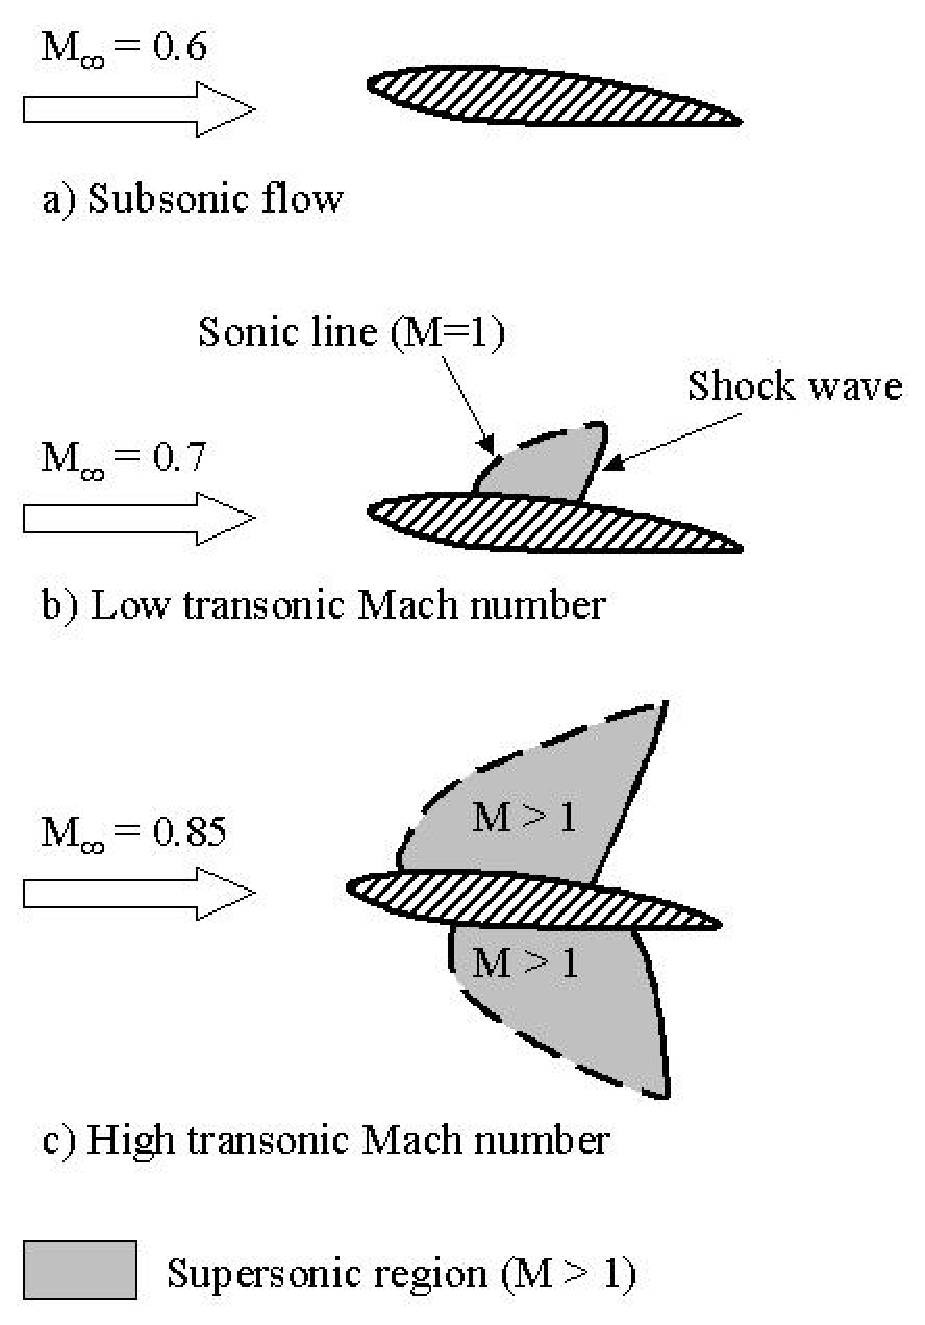
\includegraphics[bb = 92 86 545 742, height=6in]{aflow}
%    \fi
%    \caption{Airfoil Picture}
%    \label{FigAir}
%  \end{center}
%\end{figure}

% above code has been macro-fied in Classes/MacroFile.tex file
%\InsertFig{\IncludeGraphicsH{aflow}{6in}{92 86 545 742}}{Airfoil Picture}{FigAir}

%So as we have now labelled it we can reference it, like so (\ref{FigAir}) and it
%is on Page \pageref{FigAir}. And as we can see, it is a very nice picture and we
%can talk about it all we want and when we are tired we can move on to the next
%chapter ...
%
%I would also like to add an extra bookmark in acroread like so ...
%\ifpdf
%  \pdfbookmark[2]{bookmark text is here}{And this is what I want bookmarked}
%\fi
% ------------------------------------------------------------------------


%%% Local Variables: 
%%% mode: latex
%%% TeX-master: "../thesis"
%%% End: 


%Materials & methods
\section{Materials \& Methods}

\subsection{Animals}
15 male VIP-deficient mice and their male WT littermates will be used. The VIP gene disruption was realised as described by Colwell et al., 2003. A neomycin resistance cassette was entered in exon four of the VIP gene of embryonic stem cells. Homologous recombinant clones were then injected into C57BL/6 blastocysts after which the blastocysts were placed in the uteri of pseudo-pregnant female mice. Chimeric offspring was then bred with C57BL/6 females.

\subsection{Surgery}
A mixture of ketamine, xylazine and atropine will be used as general anaesthetic and lidocaine will be used as a local analgesic. A buprenorphine (Temgesic) will be administered as a postoperative analgesic. Electrode implantation will be achieved by fixating the animal's head in a stereotact and using the skull suture intersections bregma and lambda as reference points. Three small screws will be fastened into the skull around the electrode entry point for docking the electrode base. The electrode will be lowered into the brain at an angle of 5∞, 0 mm cranial to bregma and -0.61 mm lateral to bregma. The electrode will be lowered down to the SCN area at -5.38 mm ventral to the entry site into the dura mater. Finally, the electrode base will be docked to the three screws with a light weight acrylic resin. The animal will be left to recover for a week  before starting any measurements.

\subsection{Measurements and analysis}
Measurements and analysis. The electrodes implanted in the animals will be connected to a setup in such a way that the animals can move freely. The signal picked up by the electrode will be sent through an amplifier to a computer, where the data will be stored for later offline analysis. The animal cages will be equipped with sensors to detect movement and drinking activity. All measurements will be recorded automatically by our internally developed software program Circa, version 1.9, and by Spike2, version 6.05a (2007), Cambridge Electronic Design. Analysis of the electrophysiological data will be performed using Igor Pro version 6.2.2.2, WaveMetrics Inc., Oregon, USA and MATLAB R2007b version 7.5.0.342, The Math Works Inc. Statistical analysis will be performed with student t-tests and one-way ANOVAs using SPSS PASW Statistics, release 17.0.2, WinWrap Basic, Polar Engineering and Consulting. 

\subsection{Histology}
Histology. A small current will be sent down the implanted electrodes to mark the location of the electrode tip. Animal brains will be extracted and brain slices will be made with cryostat sectioning. Cresyl blue stainings will be performed to visualise brain structures and identify the electrode tip location.

%Results
\section{Results}

Results!

%Discussion
\section{Discussion}

Discuss stuff!

%Conclusion
\section{Conclusion}

Conclusion!
}
\end{multicols}
\chapter{My Second Chapter}
\ifpdf
    \graphicspath{{Chapter2/Chapter2Figs/PNG/}{Chapter2/Chapter2Figs/PDF/}{Chapter2/Chapter2Figs/}}
\else
    \graphicspath{{Chapter2/Chapter2Figs/EPS/}{Chapter2/Chapter2Figs/}}
\fi

\section{First Section}
\markboth{\MakeUppercase{\thechapter. My Second Chapter }}
And now I begin my second chapter here ...

\section{Second Section}
\markboth{\MakeUppercase{\thechapter. My Second Chapter }}
and here I write more ...

\subsection{first subsection in the Second Section}
... and some more ...

\subsection{second subsection in the Second Section}
... and some more ...

\subsection{third subsection in the Second Section}
... and some more ...

% ------------------------------------------------------------------------

%%% Local Variables: 
%%% mode: latex
%%% TeX-master: "../thesis"
%%% End: 

\chapter{My Third Chapter}
\ifpdf
    \graphicspath{{Chapter3/Chapter3Figs/PNG/}{Chapter3/Chapter3Figs/PDF/}{Chapter3/Chapter3Figs/}}
\else
    \graphicspath{{Chapter3/Chapter3Figs/EPS/}{Chapter3/Chapter3Figs/}}
\fi

\section{First Section of the Third Chapter}
\markboth{\MakeUppercase{\thechapter. My Third Chapter }}{\thechapter. My Third Chapter}
And now I begin my third chapter here ...

\subsection{first subsection in the First Section}
... and some more 

\subsection{second subsection in the First Section}
... and some more ...

\subsubsection{first subsub section in the second subsection}
... and some more in the first subsub section otherwise it all looks the same
doesn't it? well we can add some text to it ...

\subsection{third subsection in the First Section}
... and some more ...

\subsubsection{first subsub section in the third subsection}
... and some more in the first subsub section otherwise it all looks the same
doesn't it? well we can add some text to it and some more and some more and
some more and some more and some more and some more and some more ...

\subsubsection{second subsub section in the third subsection}
... and some more in the first subsub section otherwise it all looks the same
doesn't it? well we can add some text to it ...

\section{Second Section of the Third Chapter}
\markboth{\MakeUppercase{\thechapter. My Third Chapter }}{\thechapter. My Third Chapter}
and here I write more ...

% ------------------------------------------------------------------------


%%% Local Variables: 
%%% mode: latex
%%% TeX-master: "../thesis"
%%% End: 

\section{Conclusions}
\label[com]{sec:conclusions}

Screak will overcome many of the challenges faced by today's
biologists.  Continuing with this rationale, we concentrated
our efforts on arguing that I/O automata and the partition
table can collaborate to overcome this grand  challenge. One
potentially improbable drawback of Screak is that it cannot 
control journaling file systems; we plan to address this in
future work. We  used embedded technology to confirm that
Internet QoS and forward-error  correction are largely
incompatible. 
 
some-more stuff \e


% Some comments

some long text line more somre SSSS somre Some may Somre
more Somre MORE TEXT some more or may some new text not wrap
but which we will comment out at some point. As we should
do. Some

some typing because I want to test the getting to the end of line which should
wrap nicely as I would wish for.

\subsubsection{conclusions subsubsection with a long title}

some text

\backmatter % book mode only
\appendix
\chapter{Appdx A}

and here I put a bit of postamble ...

% ------------------------------------------------------------------------

%%% Local Variables: 
%%% mode: latex
%%% TeX-master: "../thesis"
%%% End: 

\chapter{Appdx B}

and here I put some more postamble ...

% ------------------------------------------------------------------------

%%% Local Variables: 
%%% mode: latex
%%% TeX-master: "../thesis"
%%% End: 


\bibliographystyle{plainnat}
%\bibliographystyle{Classes/CUEDbiblio}
%\bibliographystyle{Classes/jmb}
%\bibliographystyle{Classes/jmb} % bibliography style
\renewcommand{\bibname}{References} % changes default name Bibliography to References
\bibliography{References/references} % References file

\end{document}
